\documentclass[a4paper, 12pt, titlepage]{article}
\usepackage[utf8]{inputenc}
\usepackage{geometry}
\usepackage{polski}
\usepackage{graphicx}
\usepackage{float}
\usepackage{etoolbox,refcount}
\usepackage{multicol}
\usepackage{fancyhdr}
\pagestyle{fancy}
\title{Modelowanie i symulacja serwomechanizmu liniowego i nieliniowego}
\author{Adrian Jałoszewski, Tomasz Kotowski}
\date{}
\newgeometry{left=2.5cm, right=2.5cm, bottom=2.5cm, top=2.5cm}

\begin{document}
	\maketitle
	\section{Cel ćwiczenia}
		Celem ćwiczenia jest zamodelowanie serwomechanizmu liniowego (regulator PID dla różnych nastaw) oraz nieliniowego (regulator trójpołożeniowy dla różnych wartości strefy martwej i stref histerezy)
	\section{Serwomechanizm liniowy}
		Poniższy schemat przedstawia naszą implementację treści zadania. Zamiast zastosować przełącznik ręczny postanowiliśmy, że użyjemy przełącznika reagującego na wartość pewnej zmiennej, którą ustalamy w skrypcie uruchamiającym symulację. Oprócz tego dodaliśmy zakłócenie w postaci skoku jednostkowego oraz sygnał wejściowy, który jest skokiem jednostkowym o podwojonej wartości.
		\begin{figure}[H]
			\centering
			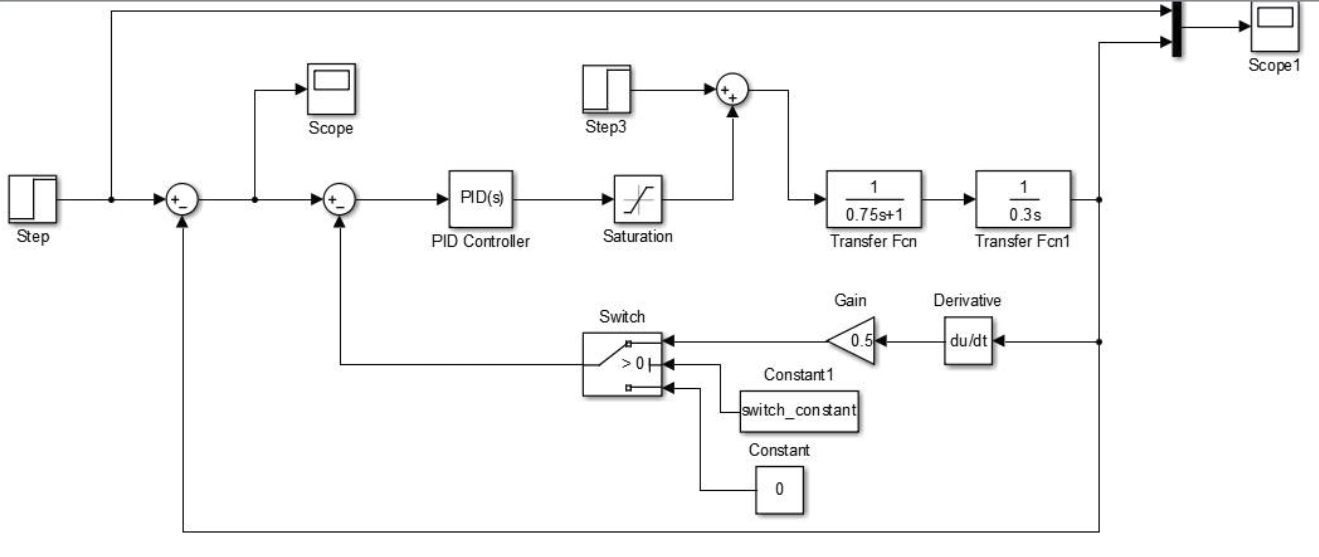
\includegraphics[width=\textwidth]{img/pid_scheme.png}
		\end{figure}
		\subsection{Regulator P}
			Przyjęliśmy regulator P z następującą transmitancją:
			$$
				G_P(s) = 2
			$$
			\subsubsection{Wyłączone sprzężenie tachometryczne}
				\begin{figure}[H]
					\centering
					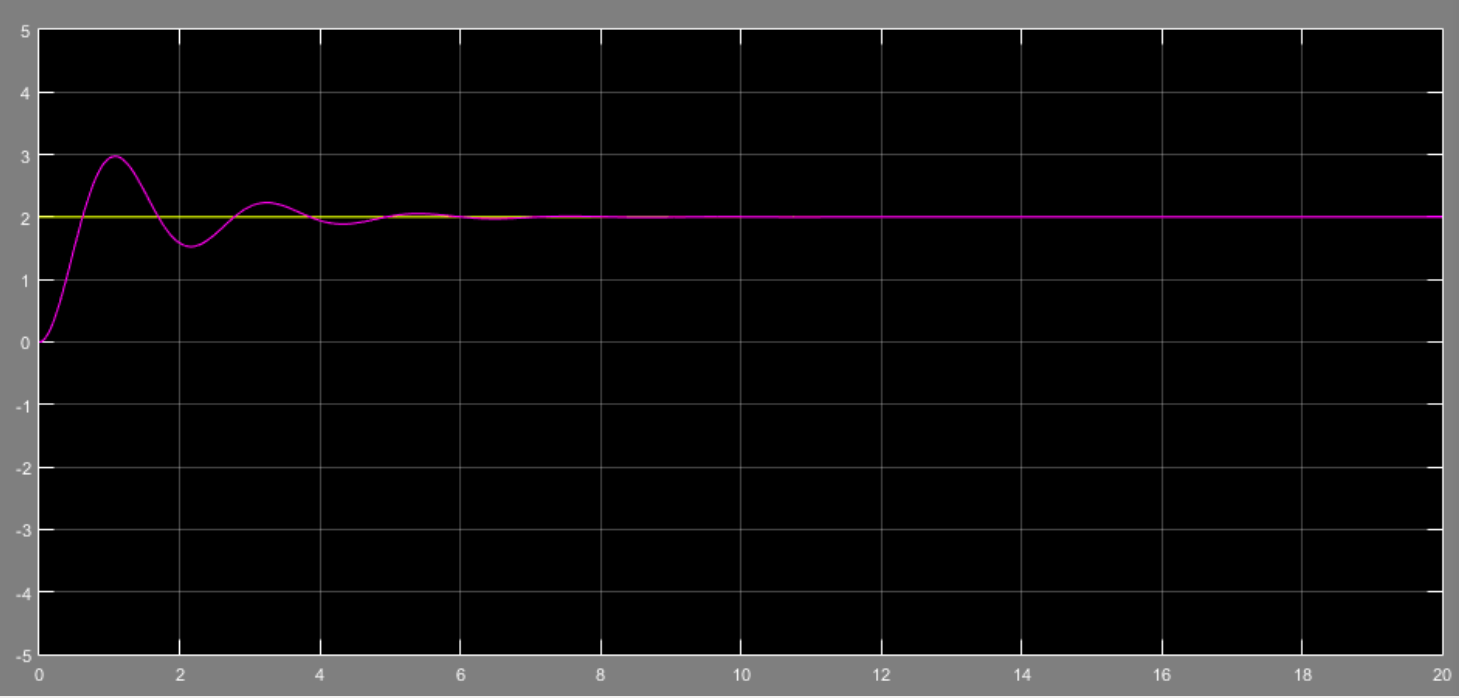
\includegraphics[width=0.7\textwidth]{img/p.png}
					\caption{Odpowiedź skokowa regulatora P}
				\end{figure}
				\begin{figure}[H]
					\centering
					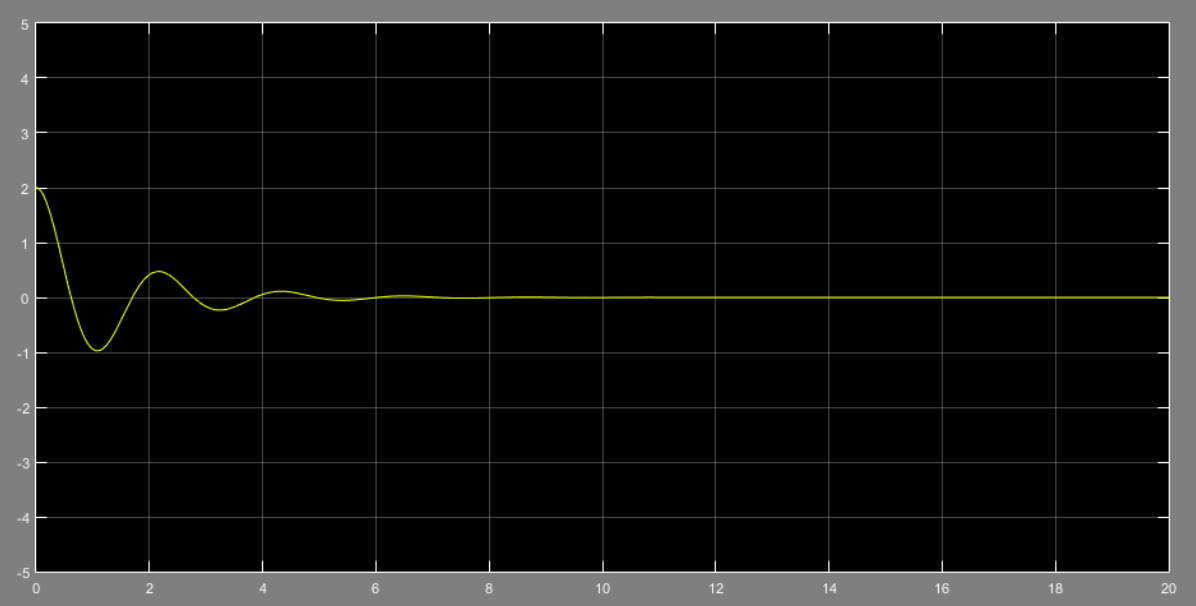
\includegraphics[width=0.7\textwidth]{img/err_p.png}
					\caption{Błąd odpowiedzi skokowej regulatora P}
				\end{figure}
				Można zauważyć na przebiegach, że serwomechanizm jako obiekt z całkowaniem niweluje uchyb ustalony -- ten spada do zera.
				\begin{figure}[H]
					\centering
					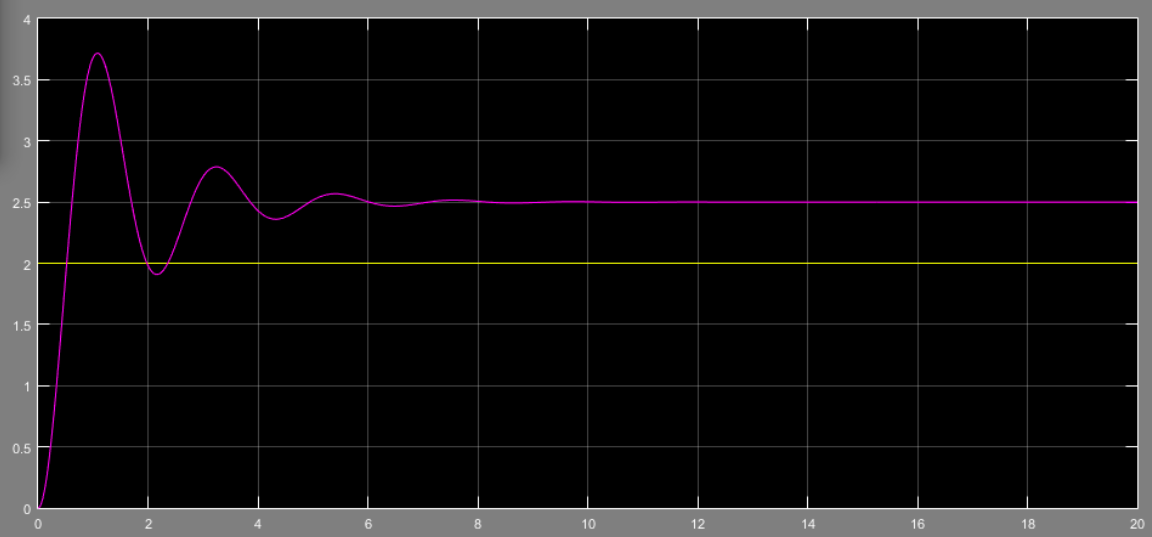
\includegraphics[width=0.7\textwidth]{img/p_noise.png}
					\caption{Odpowiedź skokowa regulatora P z zakłóceniem}
				\end{figure}
				\begin{figure}[H]
					\centering
					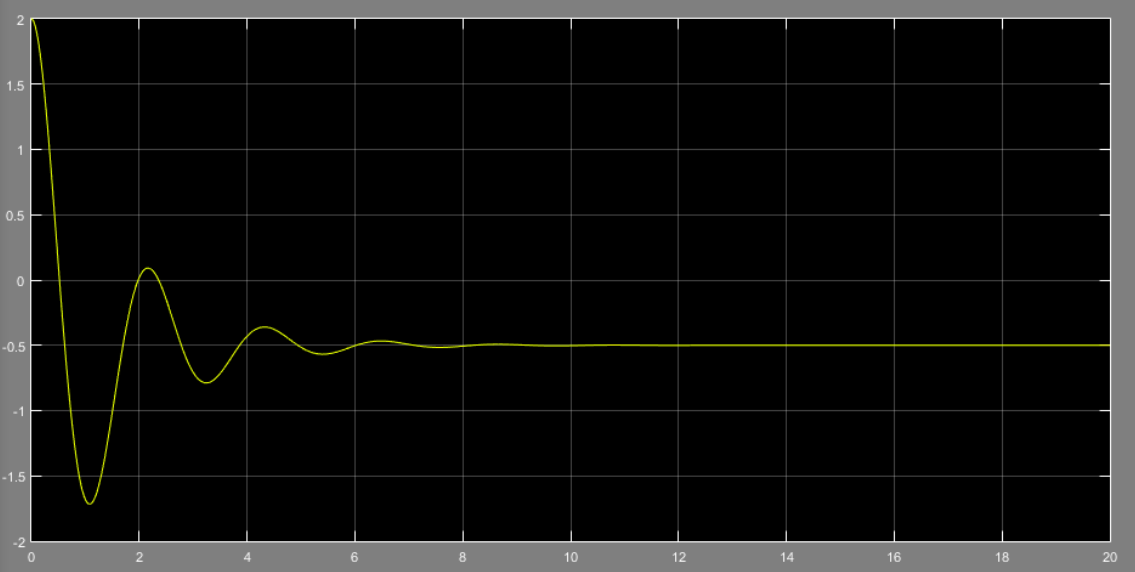
\includegraphics[width=0.7\textwidth]{img/err_p_noise.png}
					\caption{Błąd odpowiedzi skokowej regulator P z zakłóceniem}
				\end{figure} \noindent
				Można zauważyć uchyb pochodzący od zakłócenia. Jest to wartość skoku jednostkowego podanego na zakłócenie przemnożonego przez odwrotność wzmocnienia.
			\subsubsection{Włączone sprzężenie tachometryczne}
				\begin{figure}[H]
					\centering
					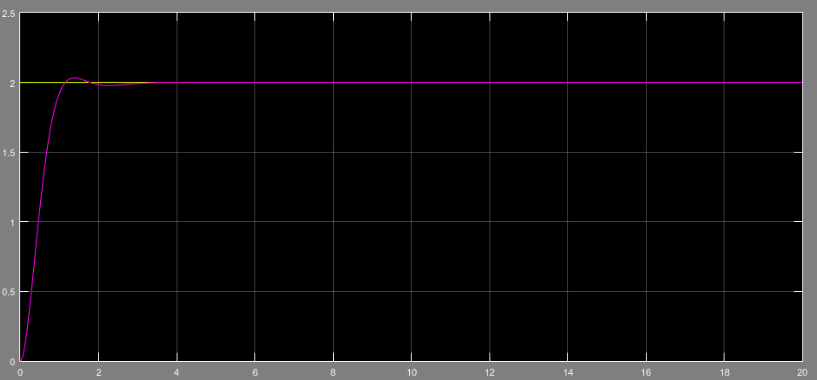
\includegraphics[width=0.7\textwidth]{img/p_tacho.png}
					\caption{Odpowiedź skokowa regulatora P ze sprzężeniem tachometrycznym}
				\end{figure}
				\begin{figure}[H]
					\centering
					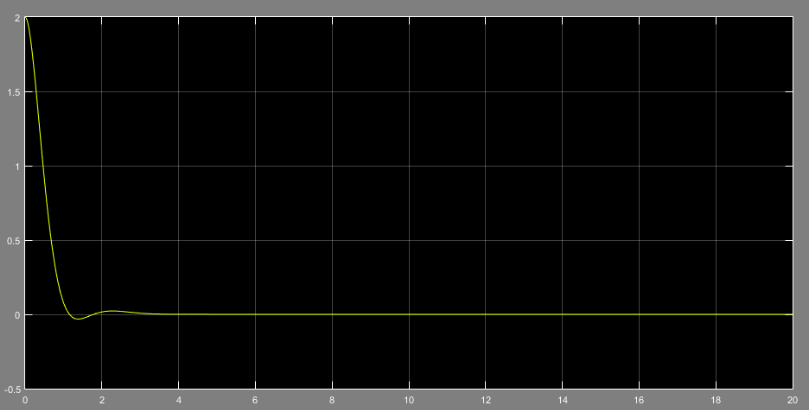
\includegraphics[width=0.7\textwidth]{img/err_p_tacho.png}
					\caption{Błąd odpowiedzi skokowej regulatora P ze sprzężeniem tachometrycznym}
				\end{figure}
				Włącznie sprzężenia tachometrycznego skutkuje poprawieniem właściwości dynamicznych układu. Układ szybciej dochodzi do stanu równowagi ze zmniejszeniem przeregulowań.
				\begin{figure}[H]
					\centering
					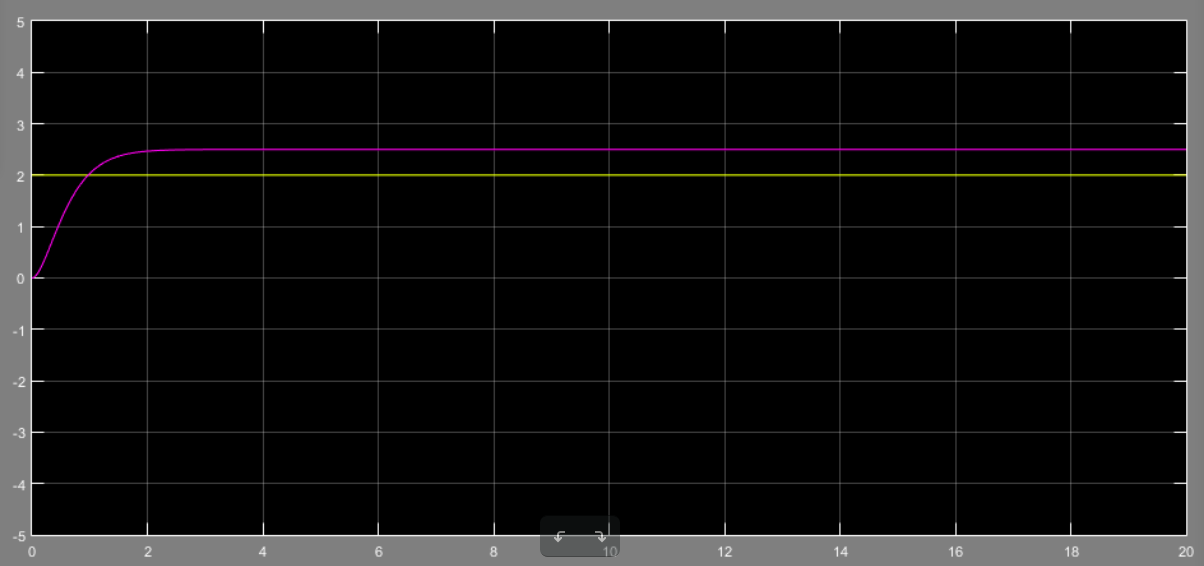
\includegraphics[width=0.7\textwidth]{img/p_noise_tacho.png}
					\caption{Odpowiedź skokowa regulatora P ze sprzężeniem tachometrycznym, z zakłóceniem}
				\end{figure}
				\begin{figure}[H]
					\centering
					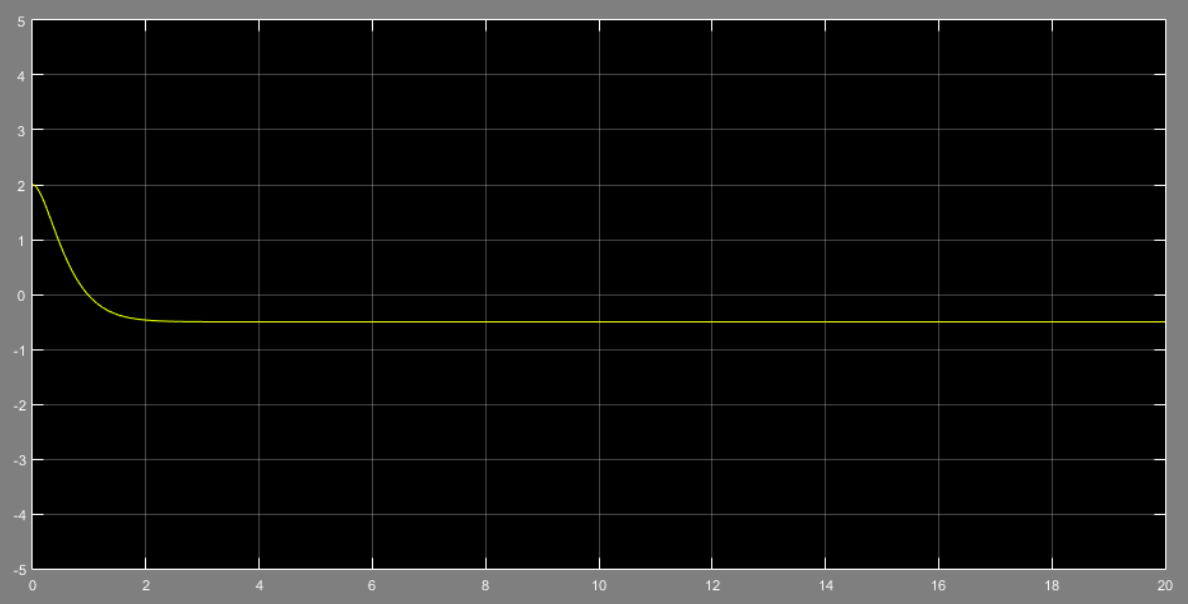
\includegraphics[width=0.7\textwidth]{img/err_p_noise_tacho.png}
					\caption{Błąd odpowiedzi skokowej regulatora P ze sprzężeniem tachometrycznym, z zakłóceniem}
				\end{figure} \noindent
				Włączenie sprzężenia tachometrycznego nie usuwa uchybu spowodowanego zakłóceniem. Ten pozostaje z tą samą wartością.
		\subsection{Regulator PI}
			W przypadku regulatora PI wybraliśmy taką transmitancję aby doprowadzić układ do stanu niestabilnego.
			$$
				G_{PI}(s) = 2 \cdot (1 + \frac{1}{s})
			$$
			\subsubsection{Wyłączone sprzężenie tachometryczne}
				Można zauważyć, że dla wybranej transmitancji układ bez sprzężenia tachometrycznego staje się niestabilny, zwiększając swoją amplitudę do nieskończoności.
				\begin{figure}[H]
					\centering
					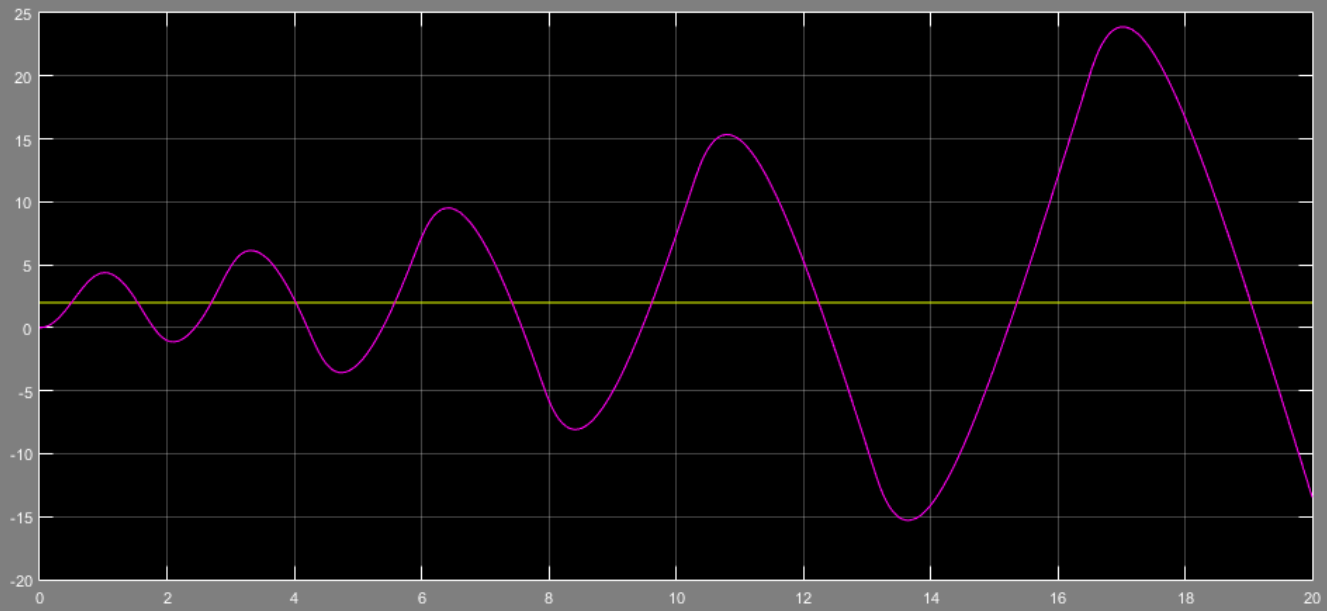
\includegraphics[width=0.7\textwidth]{img/pi.png}
					\caption{Odpowiedź skokowa regulatora PI}
				\end{figure}
				\begin{figure}[H]
					\centering
					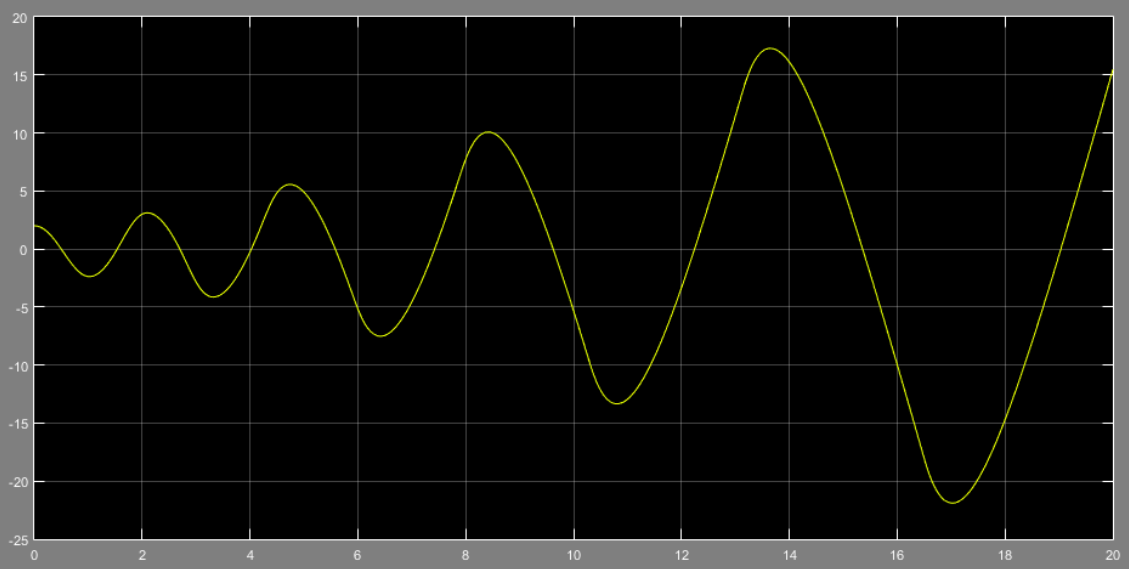
\includegraphics[width=0.7\textwidth]{img/err_pi.png}
					\caption{Błąd odpowiedzi skokowej regulatora PI}
				\end{figure}
			\subsubsection{Włączone sprzężenie tachometryczne}
				\begin{figure}[H]
					\centering
					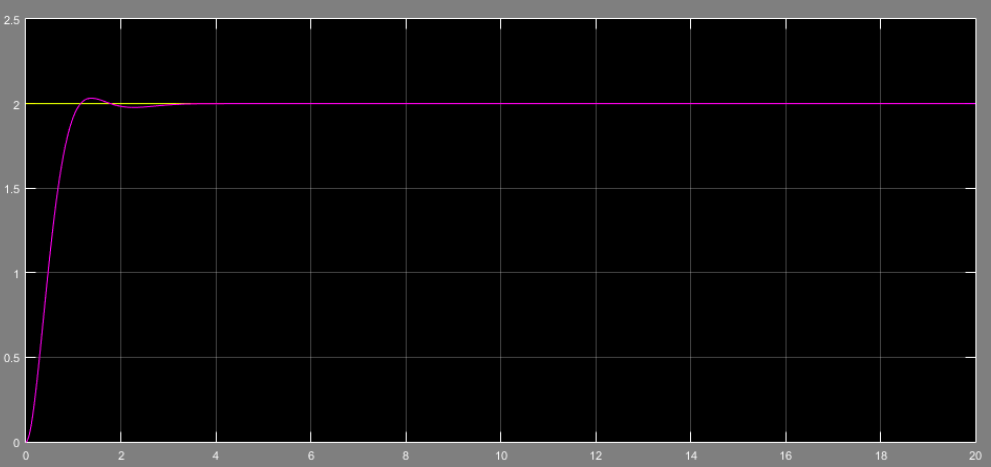
\includegraphics[width=0.7\textwidth]{img/pi_tacho.png}
					\caption{Odpowiedź skokowa regulatora PI ze sprzężeniem tachometrycznym}
				\end{figure}
				\begin{figure}[H]
					\centering
					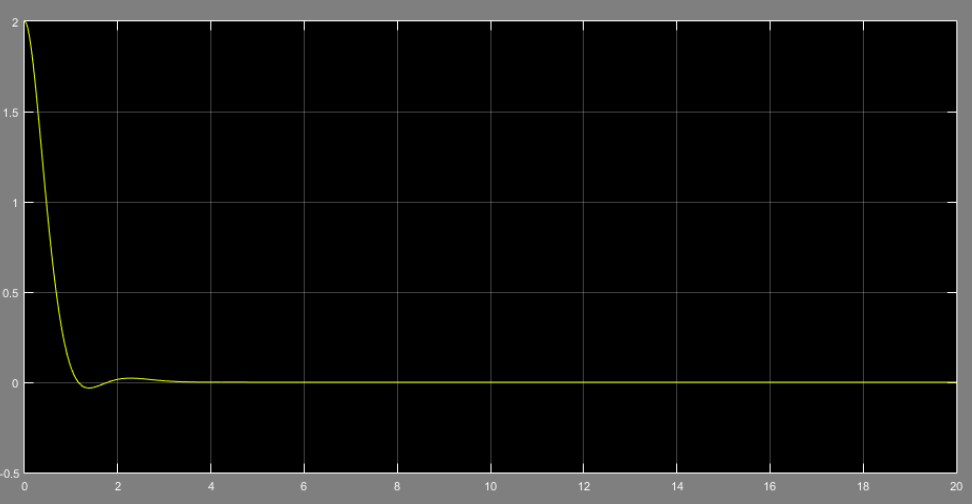
\includegraphics[width=0.7\textwidth]{img/err_pi_tacho.png}
					\caption{Błąd odpowiedzi skokowej regulatora PI ze sprzężeniem tachometrycznym}
				\end{figure}
				Można zauważyć, że wprowadzenie sprzężenia tachometrycznego pozwoliło na zachowanie stabilności układu, który był przedtem niestabilny -- polepszyło jego właściwości dynamiczne.
				\begin{figure}[H]
					\centering
					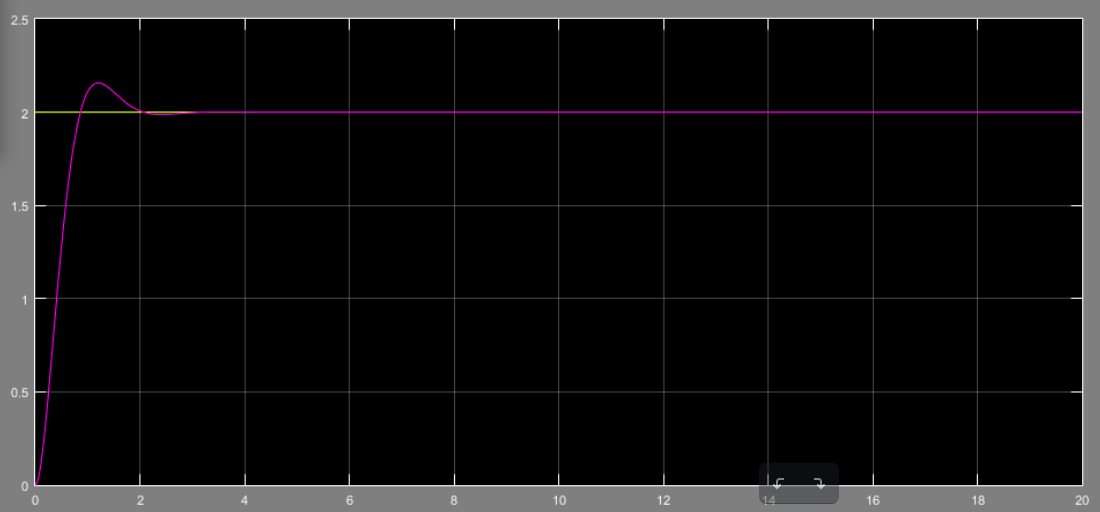
\includegraphics[width=0.7\textwidth]{img/pi_noise_tacho.png}
					\caption{Odpowiedź skokowa regulatora PI ze sprzężeniem tachometrycznym, z zakłóceniem}
				\end{figure}
				\begin{figure}[H]
					\centering
					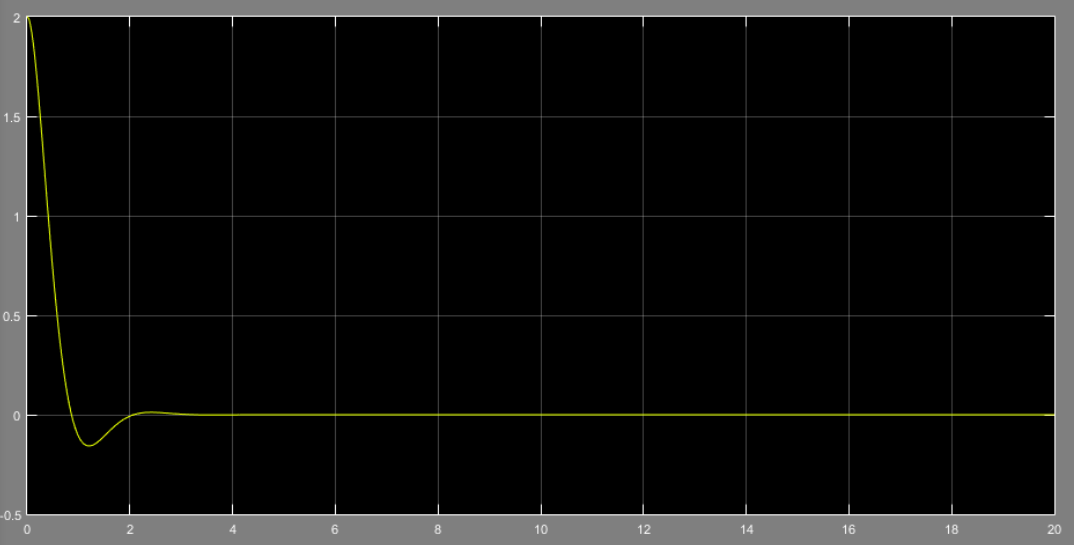
\includegraphics[width=0.7\textwidth]{img/err_pi_noise_tacho.png}
					\caption{Błąd odpowiedzi skokowej regulatora PI ze sprzężeniem tachometrycznym, z zakłóceniem}
				\end{figure} \noindent
				Wprowadzenie w regulatorze akcji całkującej usuwa uchyb ustalony wynikający z zakłócenia. Jednak pogarsza to stabilność układu ze względu na występujące podwójne całkowanie -- w regulatorze oraz w sterowanym obiekcie.
	\newpage
	\section{Serwomechanizm nieliniowy}
		Podobnie jak w przypadku serwomechanizmu liniowego tak i tutaj zmieniliśmy przełącznik ręczny na uruchamiany zadaniem wartości z poziomu skryptu. W ten sam sposób zamodelowaliśmy zakłócenie oraz w ten sam sposób przyjęliśmy wejście układu.
		\begin{figure}[H]
			\centering
			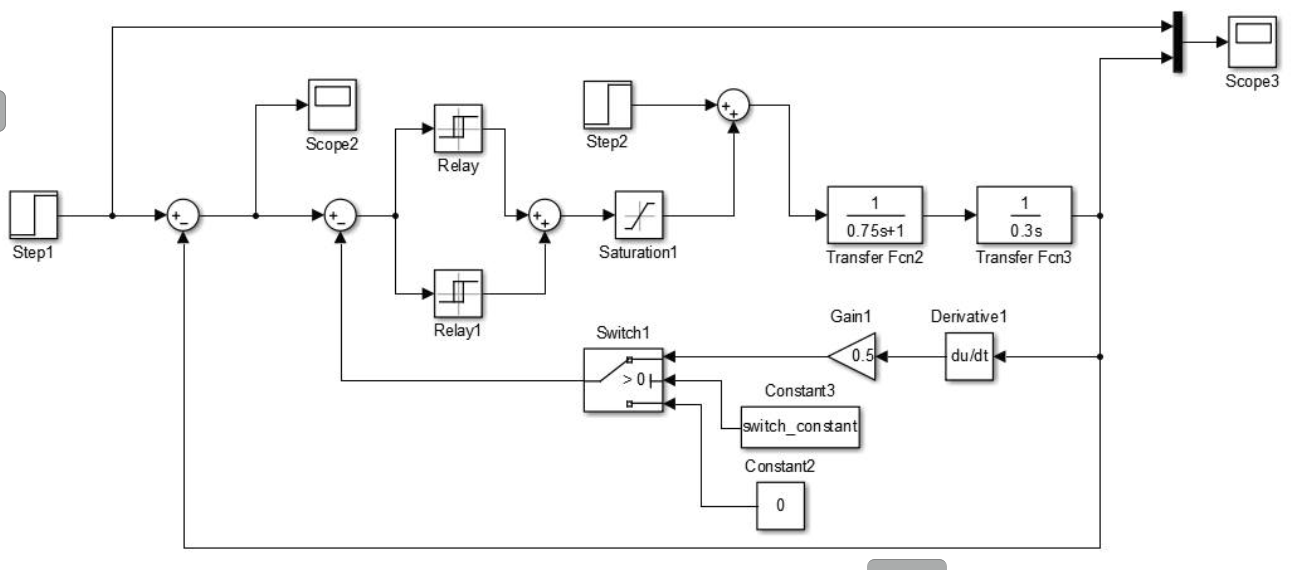
\includegraphics[width=\textwidth]{img/tri_scheme.png}
		\end{figure}
		\subsection{Regulator trójpołożeniowy}
			Do rozważań przyjęliśmy regulator trójpołożeniowy ze strefą martwą w przedziale [-0,25, 0,25] oraz strefami histerezy w przedziałach [-0,75, -0,25] (wartość -5) oraz [0,25, 0,75] (wartość 5).
			\subsubsection{Wyłączone sprzężenie tachometryczne}
				\begin{figure}[H]
					\centering
					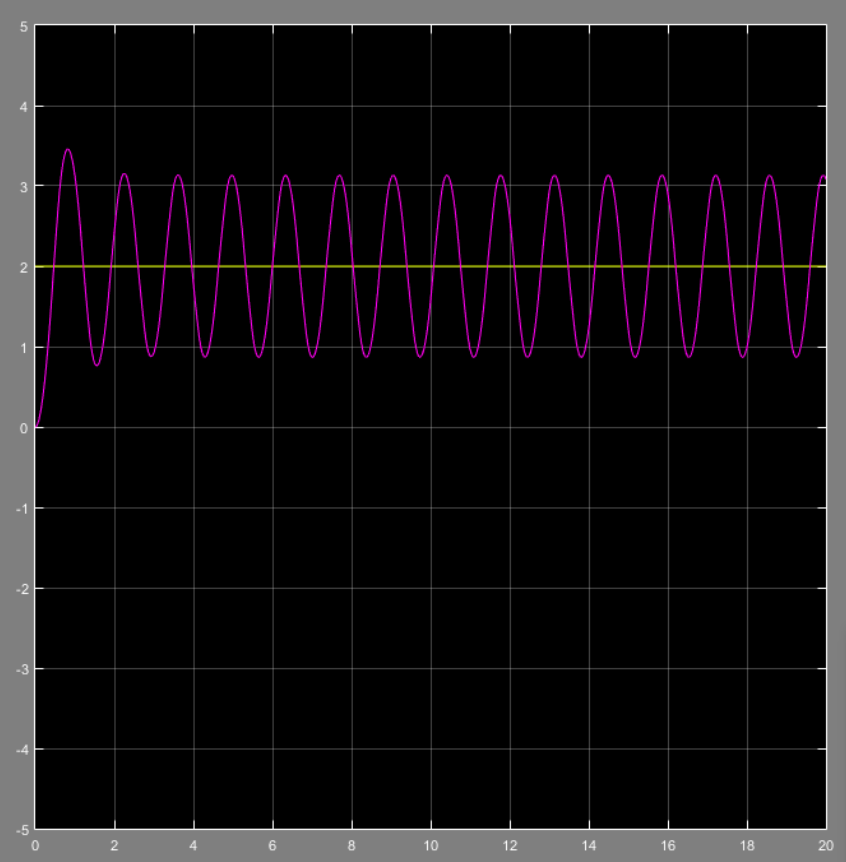
\includegraphics[width=0.55\textwidth]{img/tri.png}
					\caption{Odpowiedź skokowa regulatora trójpołożeniowego}
				\end{figure}
				\begin{figure}[H]
					\centering
					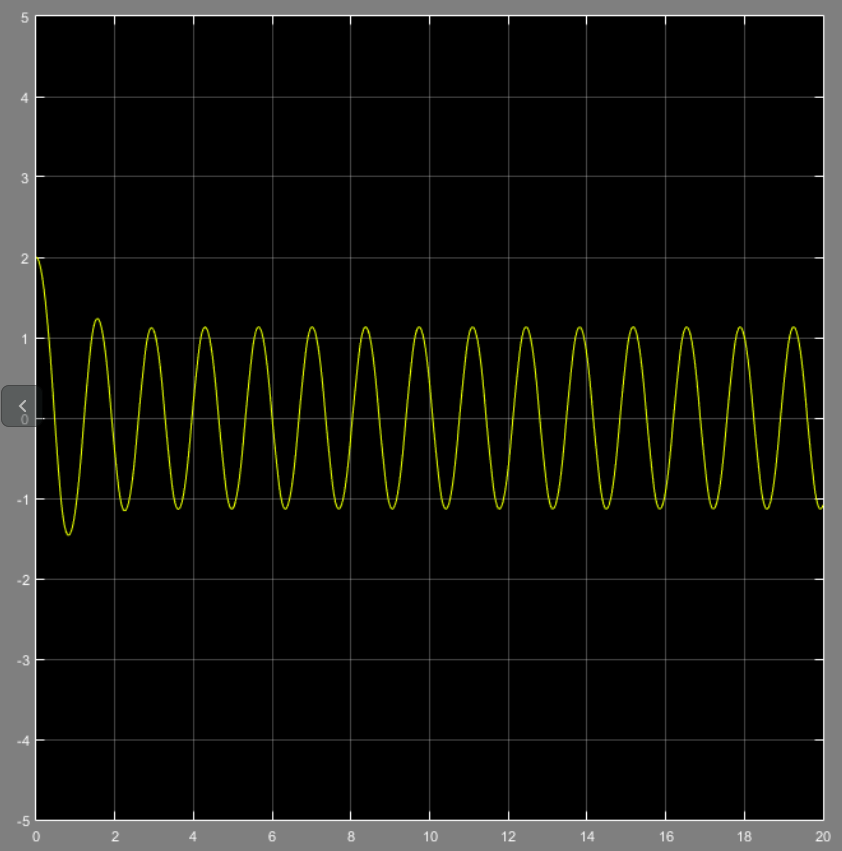
\includegraphics[width=0.55\textwidth]{img/err_tri.png}
					\caption{Błąd odpowiedzi skokowej regulatora trójpołożeniowego}
				\end{figure}
				Można zauważyć, że wartość na wyjściu oscyluje w pewnym przedziale wokół wartości zadanej -- wynika to z działania regulacji trójpołożeniowej. 
				\begin{figure}[H]
					\centering
					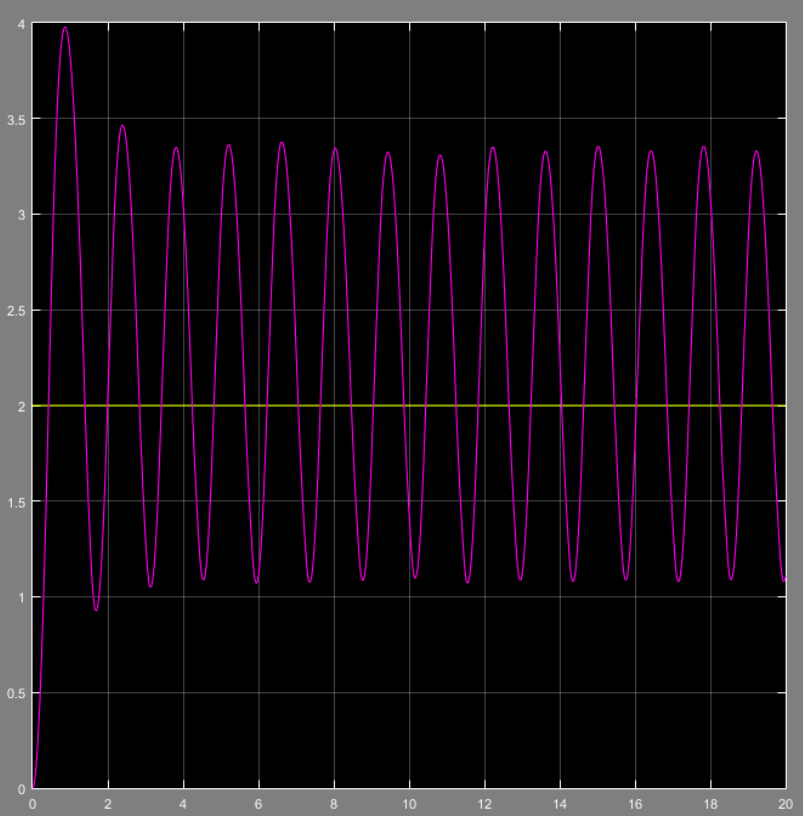
\includegraphics[width=0.55\textwidth]{img/tri_noise.png}
					\caption{Odpowiedź skokowa regulatora trójpołożeniowego z zakłóceniem}
				\end{figure}
				\begin{figure}[H]
					\centering
					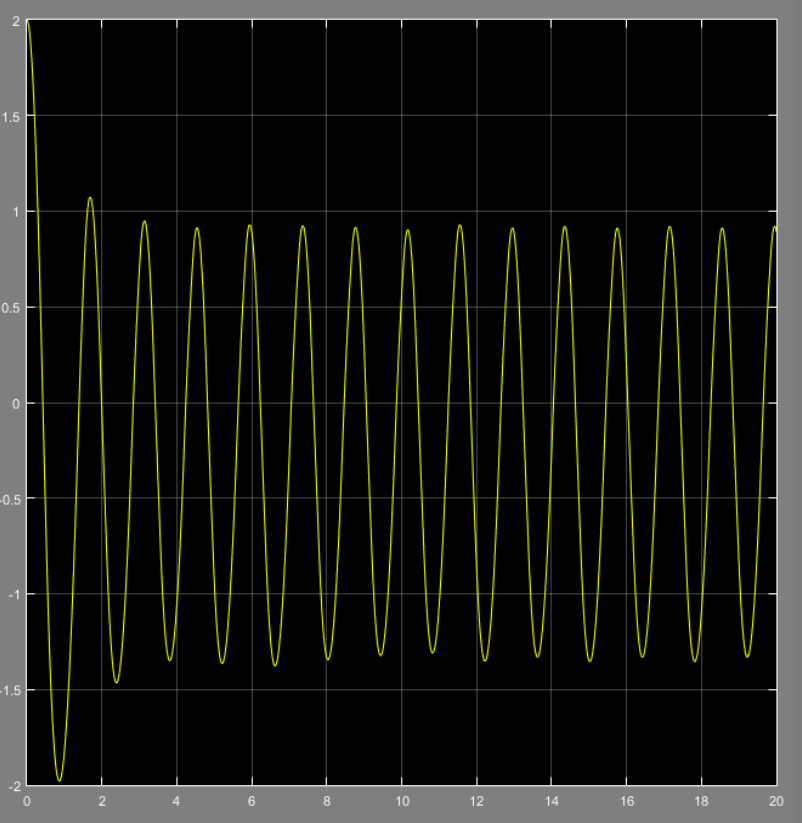
\includegraphics[width=0.55\textwidth]{img/err_tri_noise.png}
					\caption{Błąd odpowiedzi skokowej regulatora trójpołożeniowego z zakłóceniem}
				\end{figure} \noindent
				Regulacja trójpołożeniowa w przypadku zastania zakłócenia nie niweluje go. Powoduje on przesunięcie wartości amplitudy o stałą wartość.
			\subsubsection{Włączone sprzężenie tachometryczne}
				\begin{figure}[H]
					\centering
					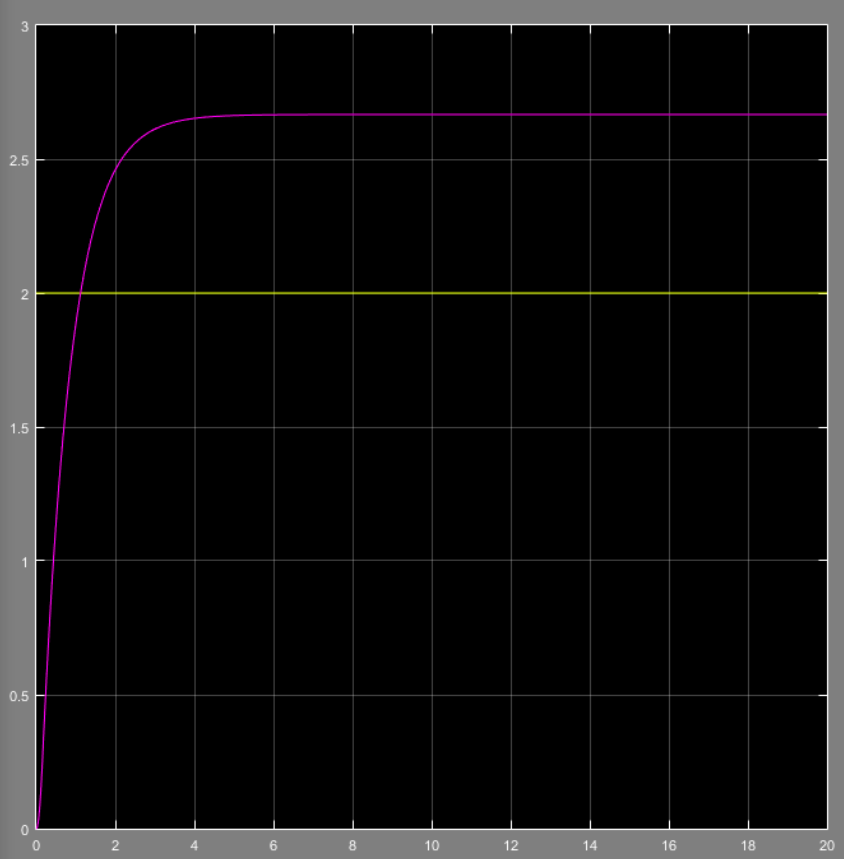
\includegraphics[width=0.55\textwidth]{img/tri_tacho.png}
					\caption{Odpowiedź skokowa regulatora trójpołożeniowego, ze sprzężeniem tachometrycznym}
				\end{figure}
				\begin{figure}[H]
					\centering
					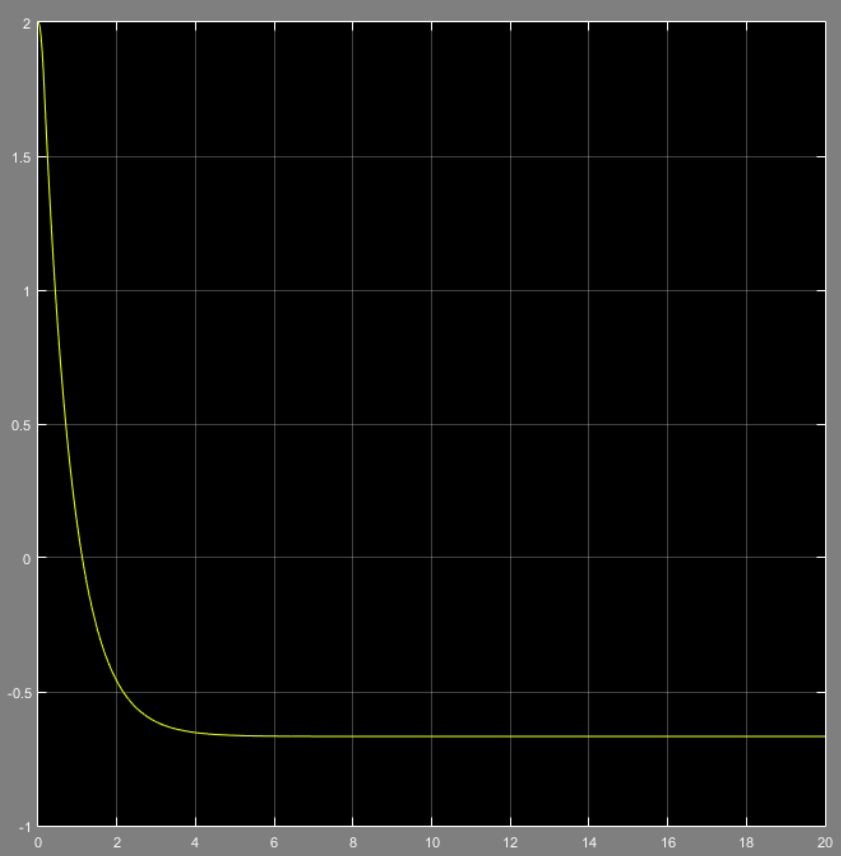
\includegraphics[width=0.55\textwidth]{img/err_tri_tacho.png}
					\caption{Błąd odpowiedzi skokowej regulatora trójpołożeniowego, ze sprzężeniem tachometrycznym}
				\end{figure}
				Można zauważyć, że oscylacje znikły, jednak układ nie osiąga wartości zadanej -- znajduje się ponad nią.
				\begin{figure}[H]
					\centering
					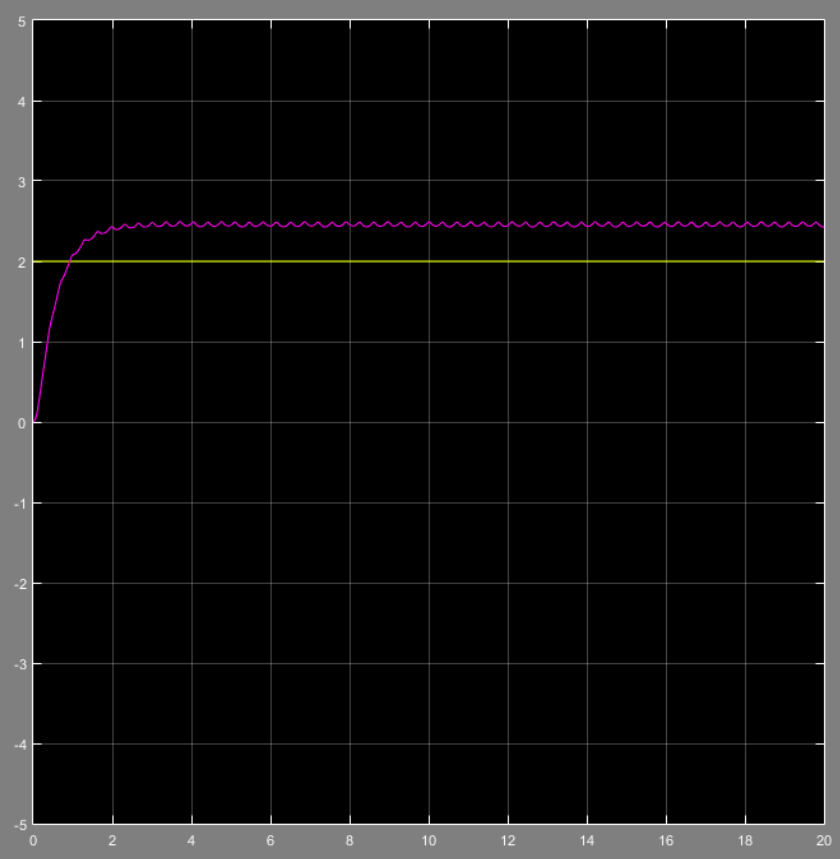
\includegraphics[width=0.55\textwidth]{img/tri_noise_tacho.png}
					\caption{Odpowiedź skokowa regulatora trójpołożeniowego, ze sprzężeniem tachometrycznym z zakłóceniem}
				\end{figure}
				\begin{figure}[H]
					\centering
					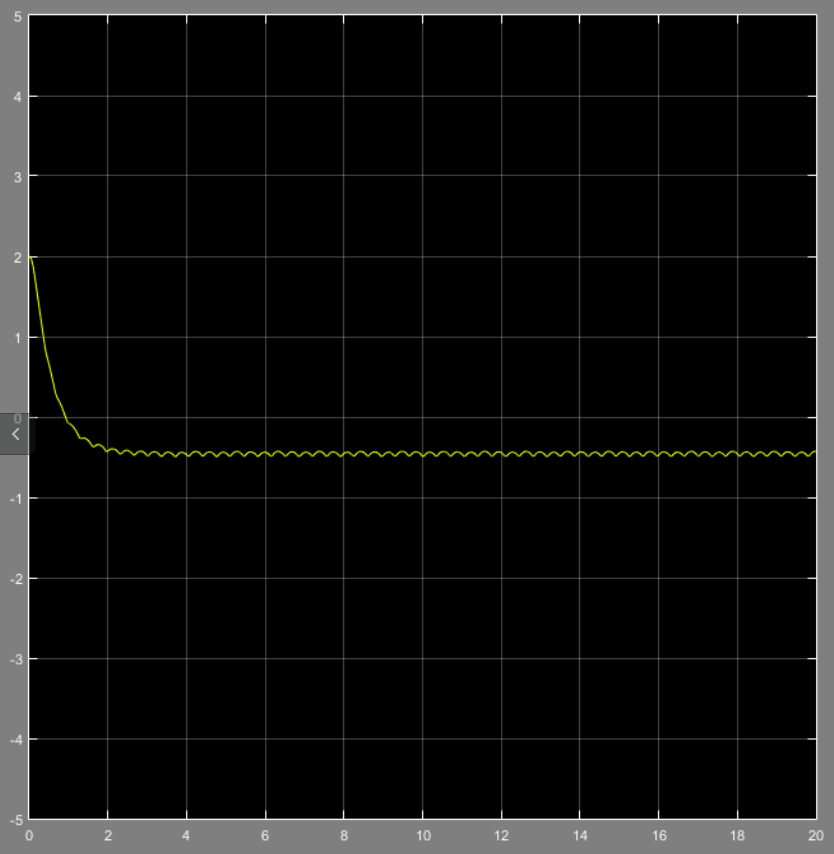
\includegraphics[width=0.5\textwidth]{img/err_tri_noise_tacho.png}
					\caption{Błąd odpowiedzi skokowej regulatora trójpołożeniowego, ze sprzężeniem tachometrycznym z zakłóceniem}
				\end{figure} \noindent
				Wprowadzenie zakłócenia do układu wprowadziło niewielkie oscylacje.
		\subsection{Regulator z zerową strefą martwą}
			Drugą wersją regulatora jaką sprawdziliśmy jest regulator z zerową strefą martwą. Przedziały w których znajduje się histereza to: [-1, 0] oraz [0, 1] odpowiednio z wartościami -5 oraz 5.
			\subsubsection{Wyłączone sprzężenie tachometryczne}
				\begin{figure}[H]
					\centering
					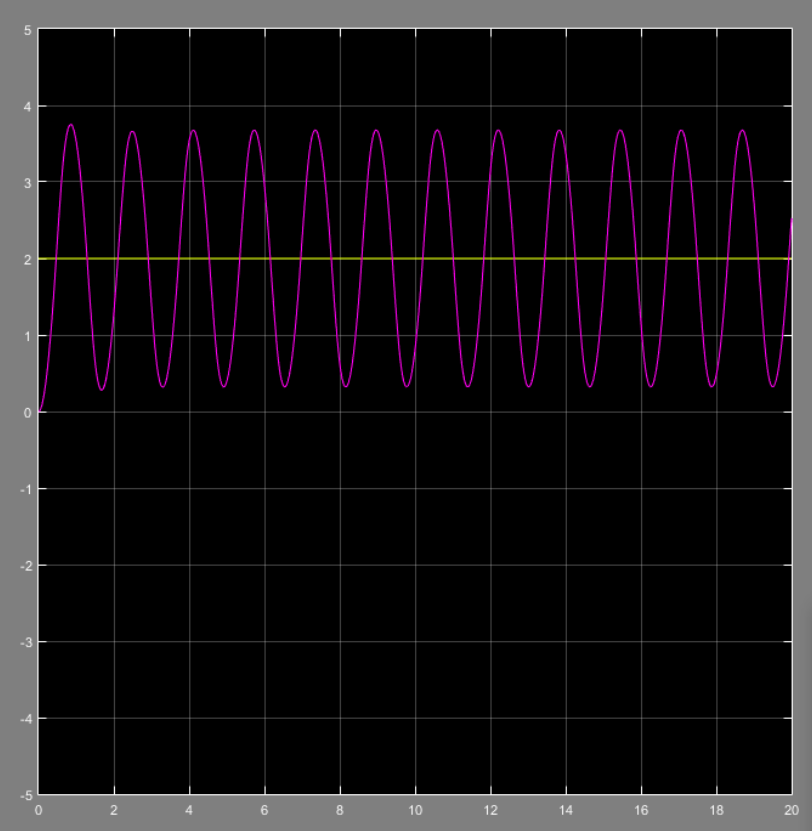
\includegraphics[width=0.5\textwidth]{img/two.png}
					\caption{Odpowiedź skokowa regulatora trójpołożeniowego z zerową strefą martwą}
				\end{figure}
				\begin{figure}[H]
					\centering
					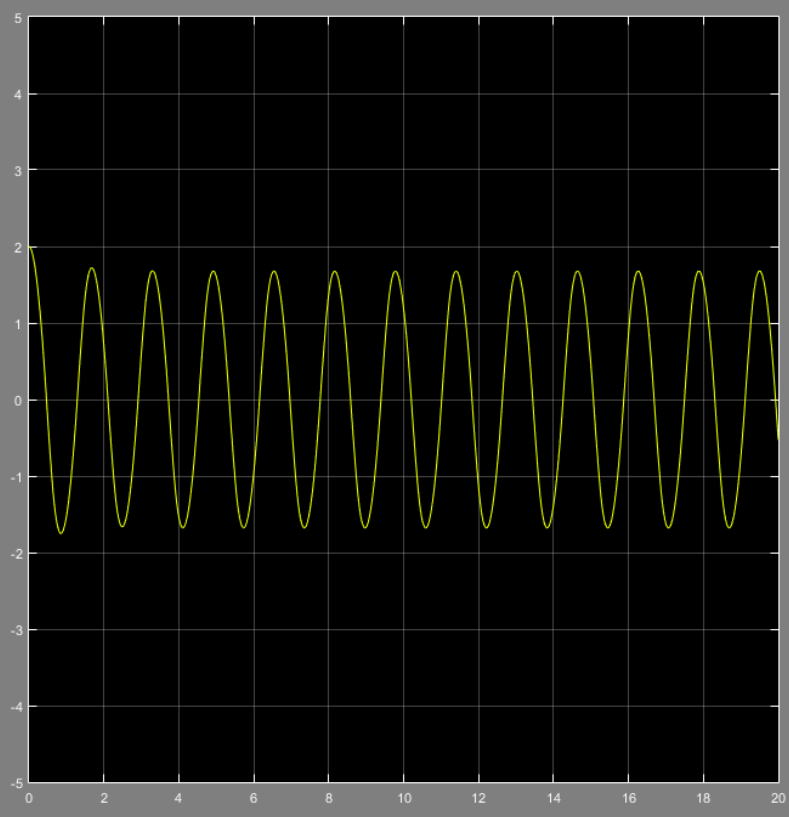
\includegraphics[width=0.5\textwidth]{img/err_two.png}
					\caption{Błąd odpowiedzi skokowej regulatora trójpołożeniowego z zerową strefą martwą}
				\end{figure}
				Układ zachowuje się tak jak w przypadku strefy martwej, jednak przesterowania są mniejsze.
				\begin{figure}[H]
					\centering
					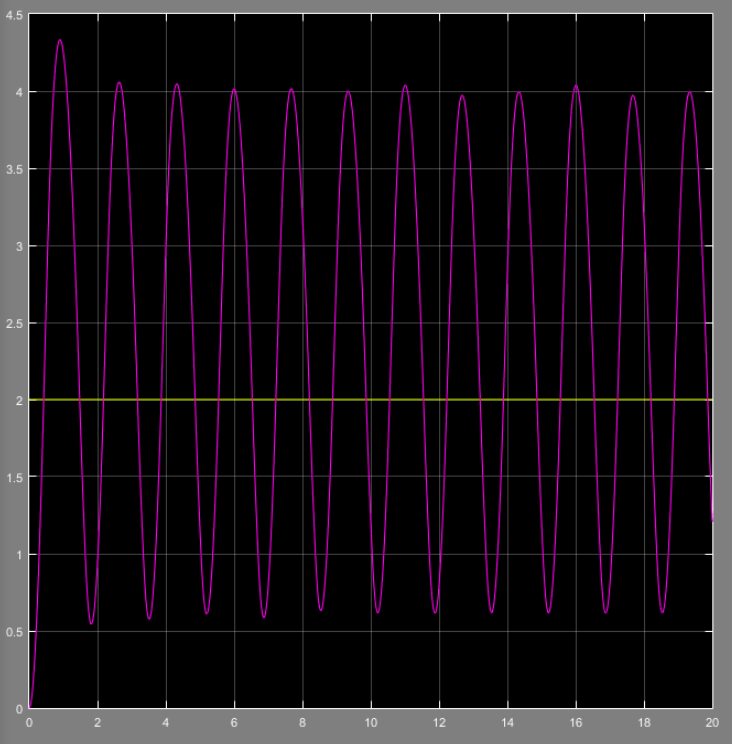
\includegraphics[width=0.5\textwidth]{img/two_noise.png}
					\caption{Odpowiedź skokowa regulatora trójpołożeniowego z zerową strefą martwą, z zakłóceniem}
				\end{figure}
				\begin{figure}[H]
					\centering
					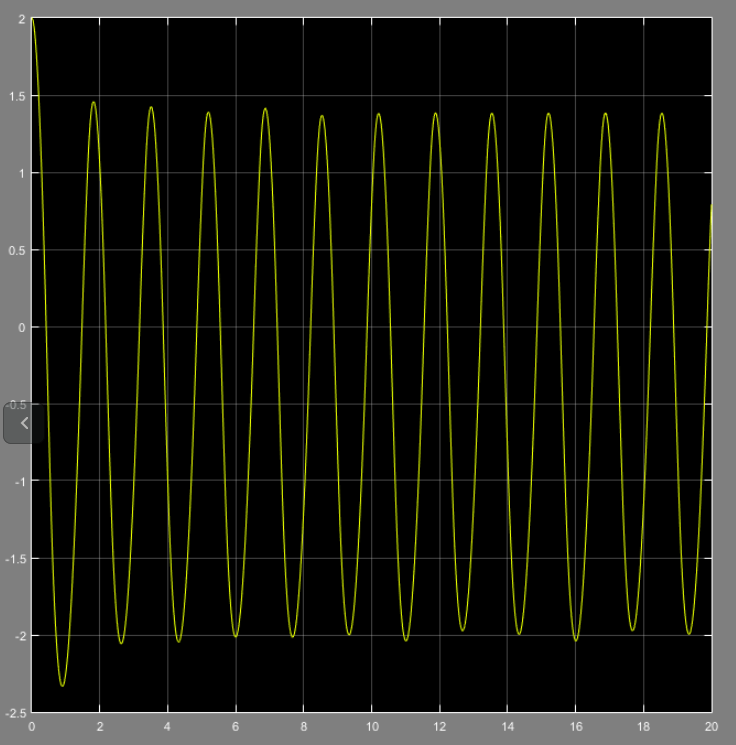
\includegraphics[width=0.5\textwidth]{img/err_two_noise.png}
					\caption{Błąd odpowiedzi skokowej regulatora trójpołożeniowego z zerową strefą martwą, z zakłóceniem}
				\end{figure} \noindent
				Układ próbuje intensywniej zwalczać zakłócenie niż w przypadku regulatora ze strefą martwą, powodując większe amplitudy oscylacji.
			\subsubsection{Włączone sprzężenie tachometryczne}
				\begin{figure}[H]
					\centering
					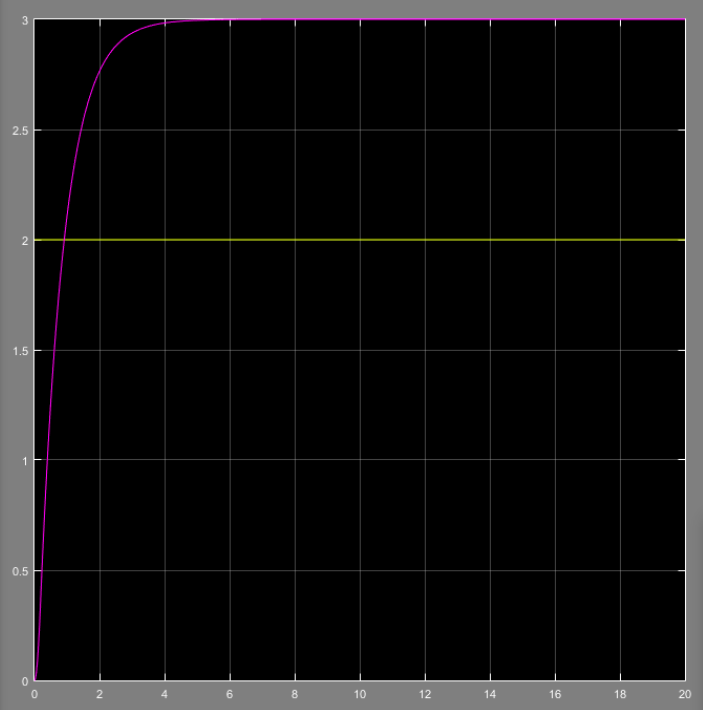
\includegraphics[width=0.5\textwidth]{img/two_tacho.png}
						\caption{Odpowiedź skokowa regulatora trójpołożeniowego z zerową strefą martwą, z włączonym sprzężeniem tachometrycznym}
				\end{figure}
				\begin{figure}[H]
					\centering
					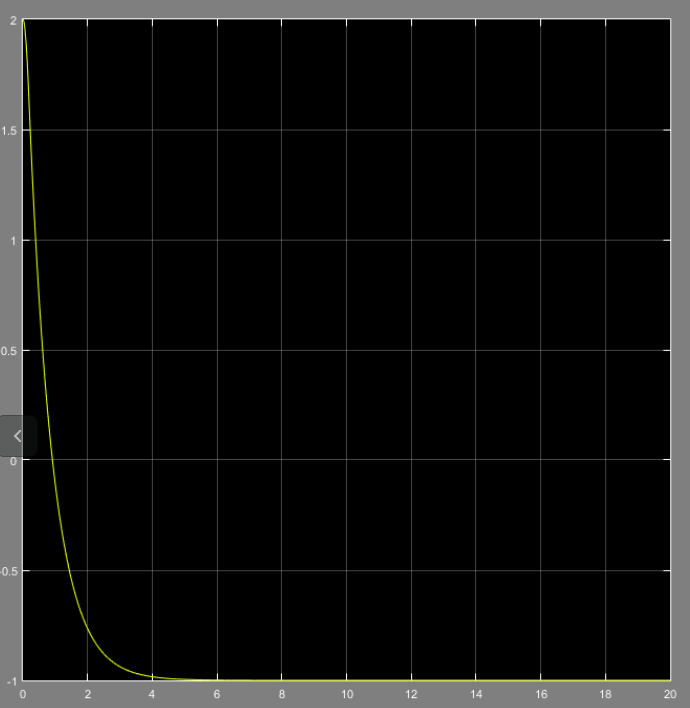
\includegraphics[width=0.5\textwidth]{img/err_two_tacho.png}
					\caption{Błąd odpowiedzi skokowej regulatora trójpołożeniowego z zerową strefą martwą, z włączonym sprzężeniem tachometrycznym}
				\end{figure}
				Zachowanie jest podobne jak dla regulatora ze strefą martwą, tyle, że występuje większe przekroczenie wartości zadanej.
				\begin{figure}[H]
					\centering
					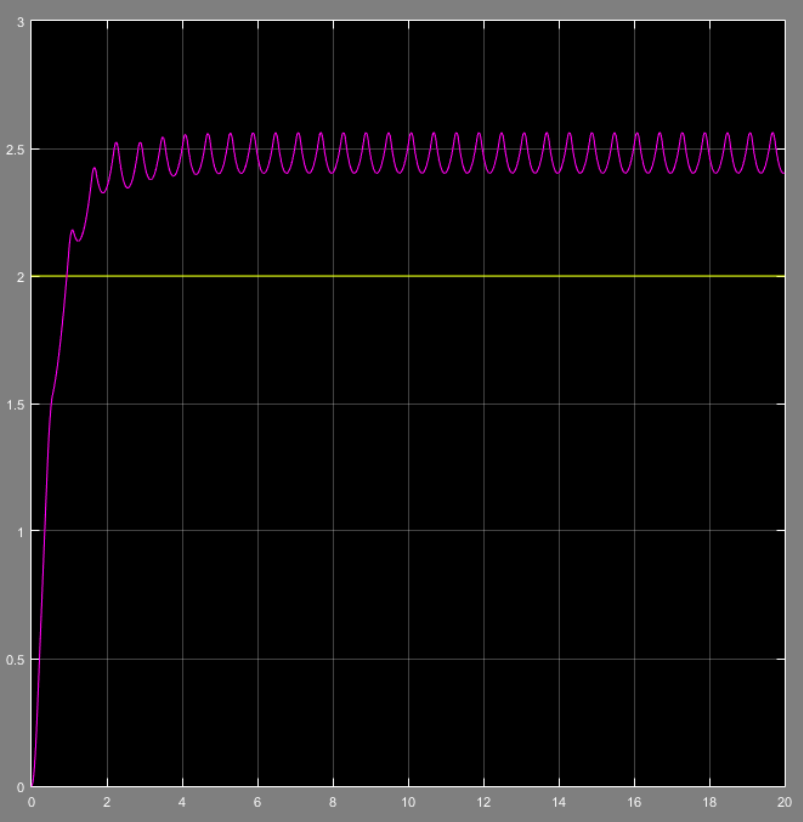
\includegraphics[width=0.5\textwidth]{img/two_noise_tacho.png}
					\caption{Odpowiedź skokowa regulatora trójpołożeniowego z zerową strefą martwą, z włączonym sprzężeniem tachometrycznym, z zakłóceniem}
				\end{figure}
				\begin{figure}[H]
					\centering
					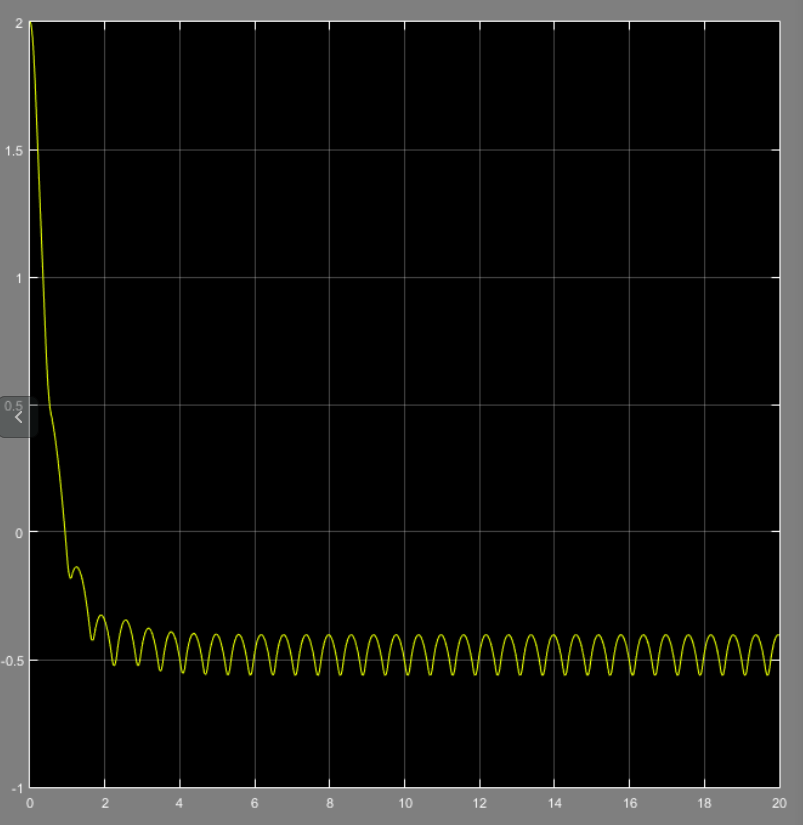
\includegraphics[width=0.5\textwidth]{img/err_two_noise_tacho.png}
					\caption{Błąd odpowiedzi skokowej regulatora trójpołożeniowego z zerową strefą martwą, z włączonym sprzężeniem tachometrycznym, z zakłóceniem}
				\end{figure} \noindent
				Można zauważyć, że układ próbuje walczyć z zakłóceniem, doprowadzając tym samym do zwiększenia oscylacji w porównaniu do tego samego przypadku, jednak ze strefą martwą.
	\section{Podsumowanie i wnioski}
		Ćwiczenie te pokazało nam jaki wpływ na dynamikę układu ma zastosowanie sprzężenia tachometrycznego. Jest ono w stanie doprowadzić układ z regulatorem PI z niestabilności do stabilności. Zastosowanie sprzężenia tachometrycznego zmniejsza również oscylacje w przypadku zastosowania regulatora trójpołożeniowego w przypadku zakłócenia oraz je kompletnie eliminuje jeżeli owego zakłócenia nie ma.
\end{document}